\chapter{Result Discussion}
 
 \section{Perturb and Observe Method }
 
 The \ac{PnO} algorithm works by periodically perturbing the cell and observing the direction of the change in power and consequently moving the $V\textsubscript{ref}$ in the same direction. The $V\textsubscript{ref}$ is moved in small increments or decrements depending on power change.
 However we soon come to realise that true \ac{MPP} is never reached and multiple iterations are required to even reach close. Due to the capacitive effect seen in \ac{DSCs}, the cells are very slow to respond to any change in operating voltage necessitating a rest period for the cells to stabilise which could vary from 500 ms to a few seconds between each step. Under such conditions the numerous iterations mandated by the \ac{PnO} method could potentially mean its several minutes before the operating point is anywhere close to the \ac{MPP}, of course assuming that the solar irradiation remains constant during this search. 
 
 The lower graph in figure~\ref{fig:PnO_result} on page~\pageref{fig:PnO_result} is the input to the model, simulating the change in incident irradiation and the top graph in blue represents input power of the solar cell. It is interesting to observe that this implementation of \ac{PnO} had trouble locking on to the \ac{MPP} during gradually incrementing light conditions.                       
  \begin{figure}[H]
	   \begin{center}
		   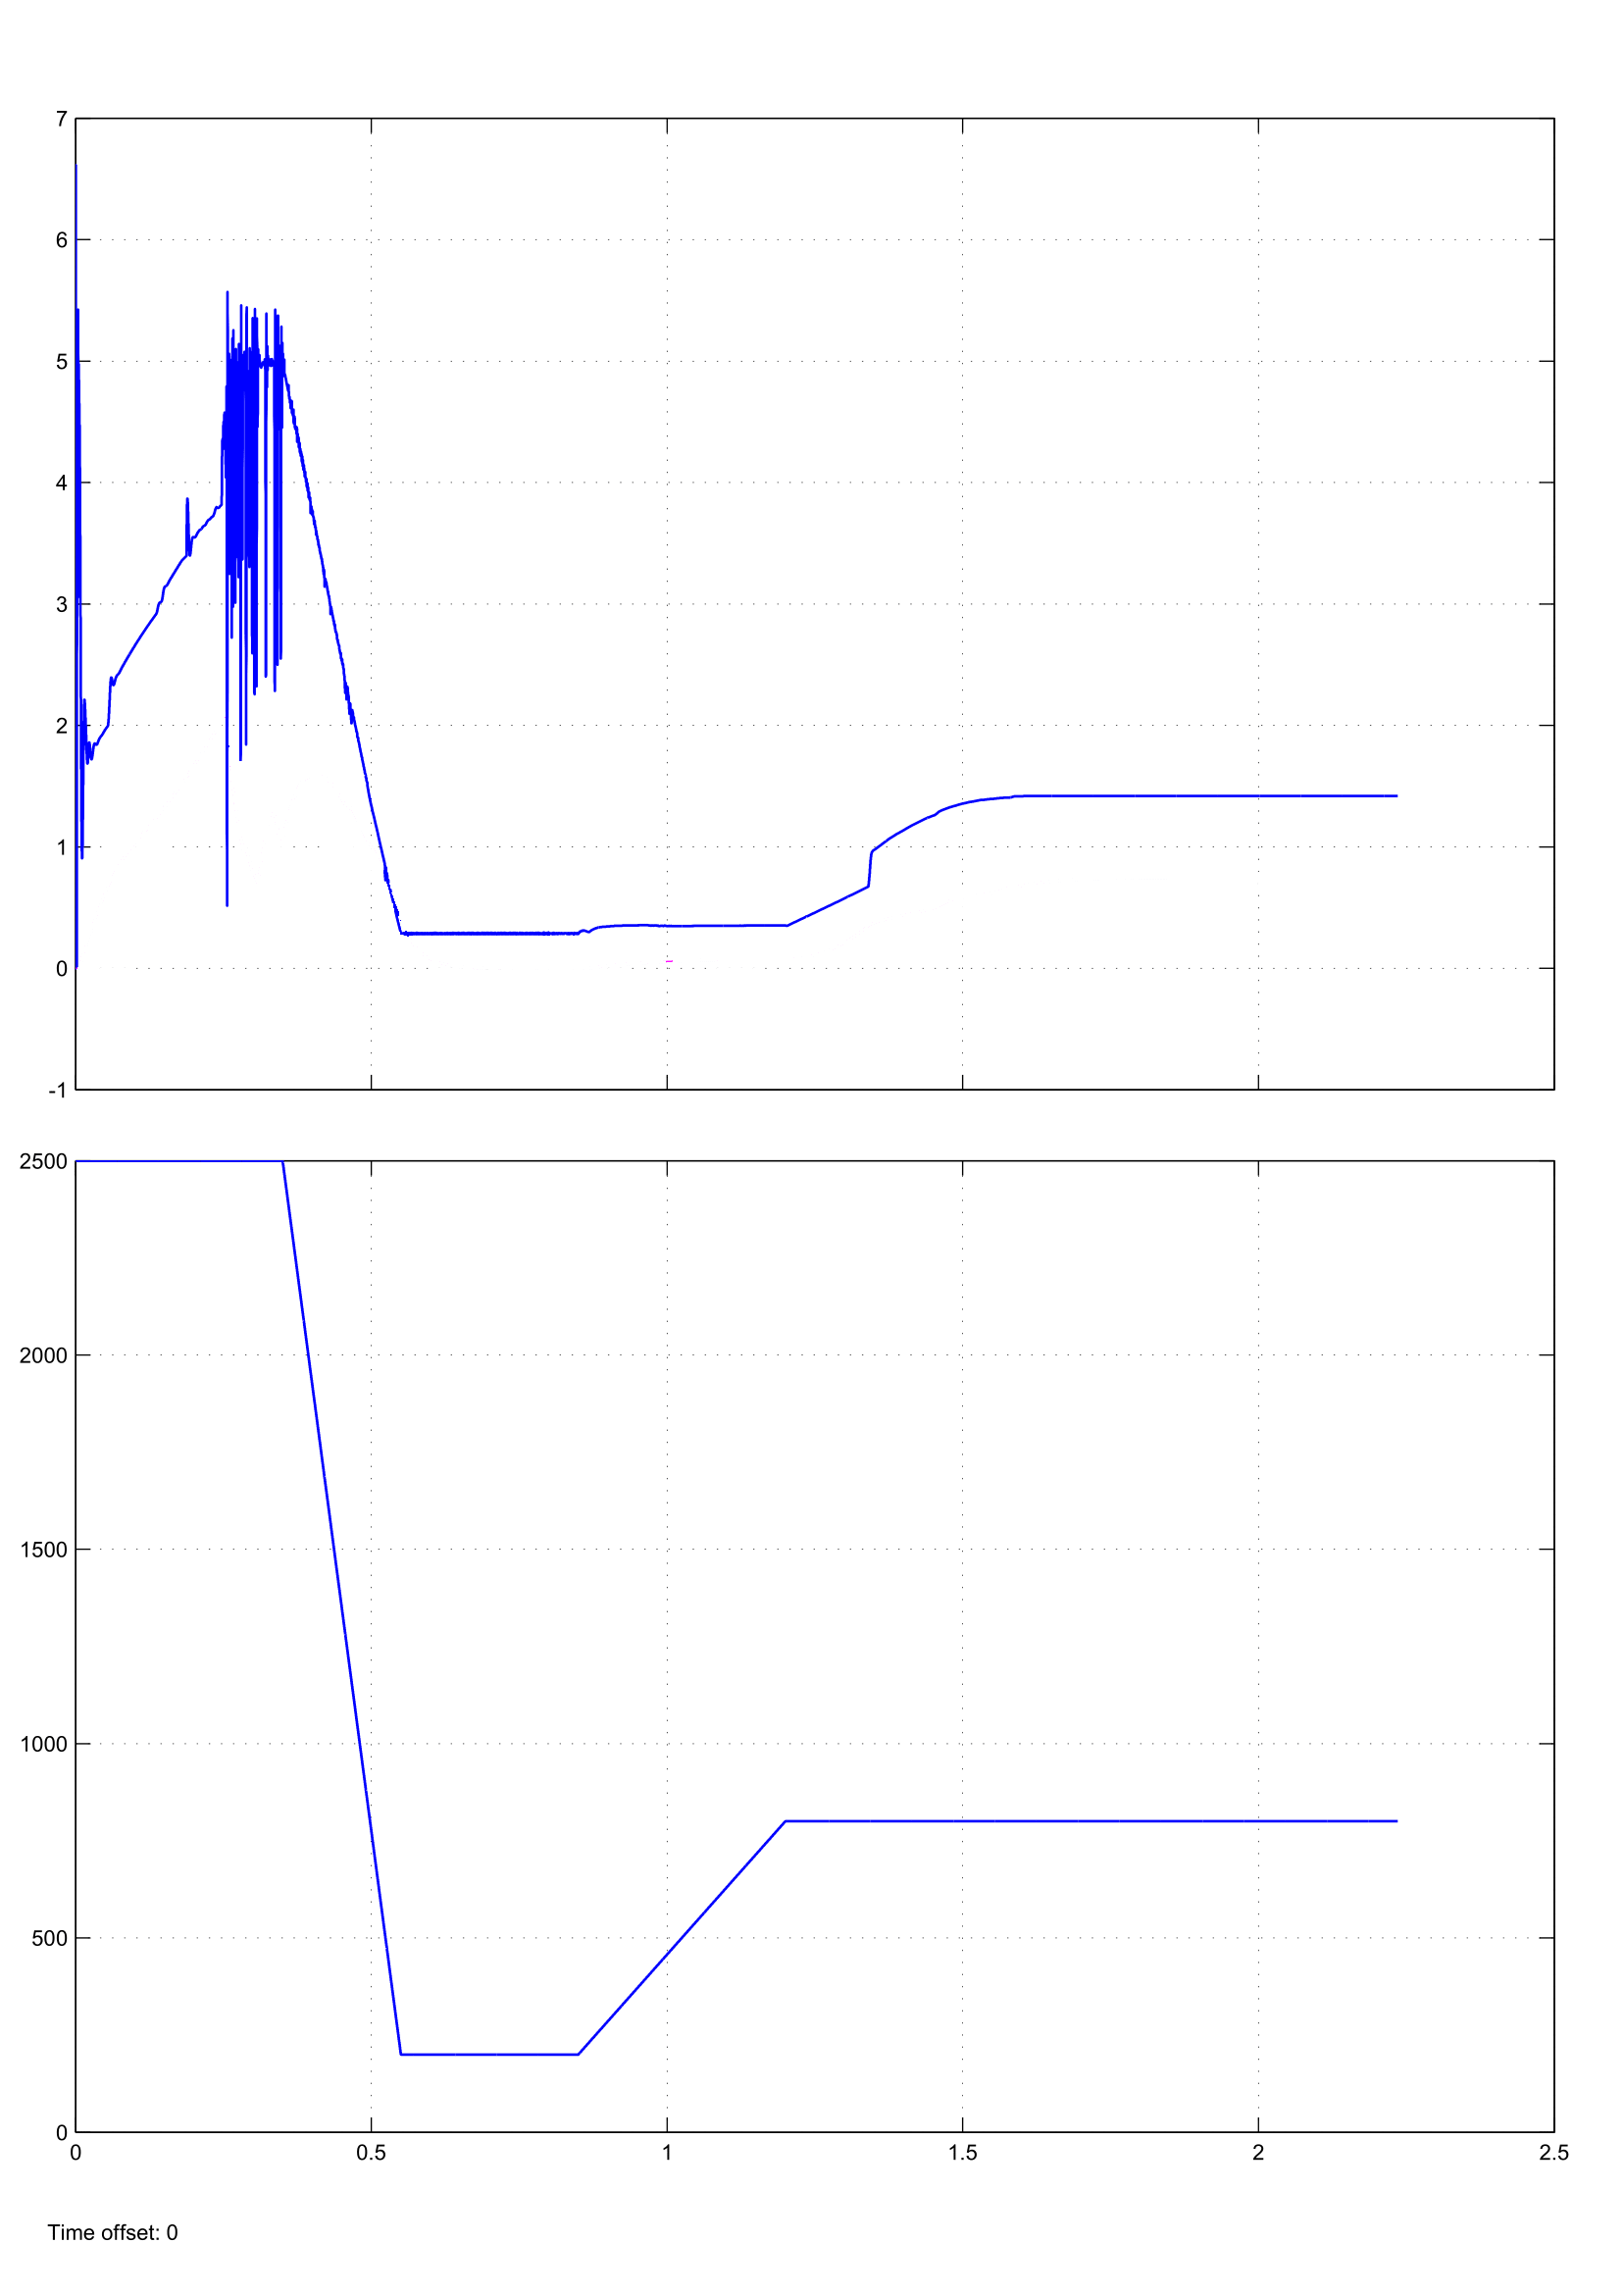
\includegraphics[width=\textwidth]{images/P&O_changing_lux-1}
		   \caption{Perturb and Observe Method on implementation   }
		   \label{fig:PnO_result}
	   \end{center}
   \end{figure}
   
 \section{Incremental Conductance Method }
 
  \begin{figure}[H]
	   \begin{center}
		   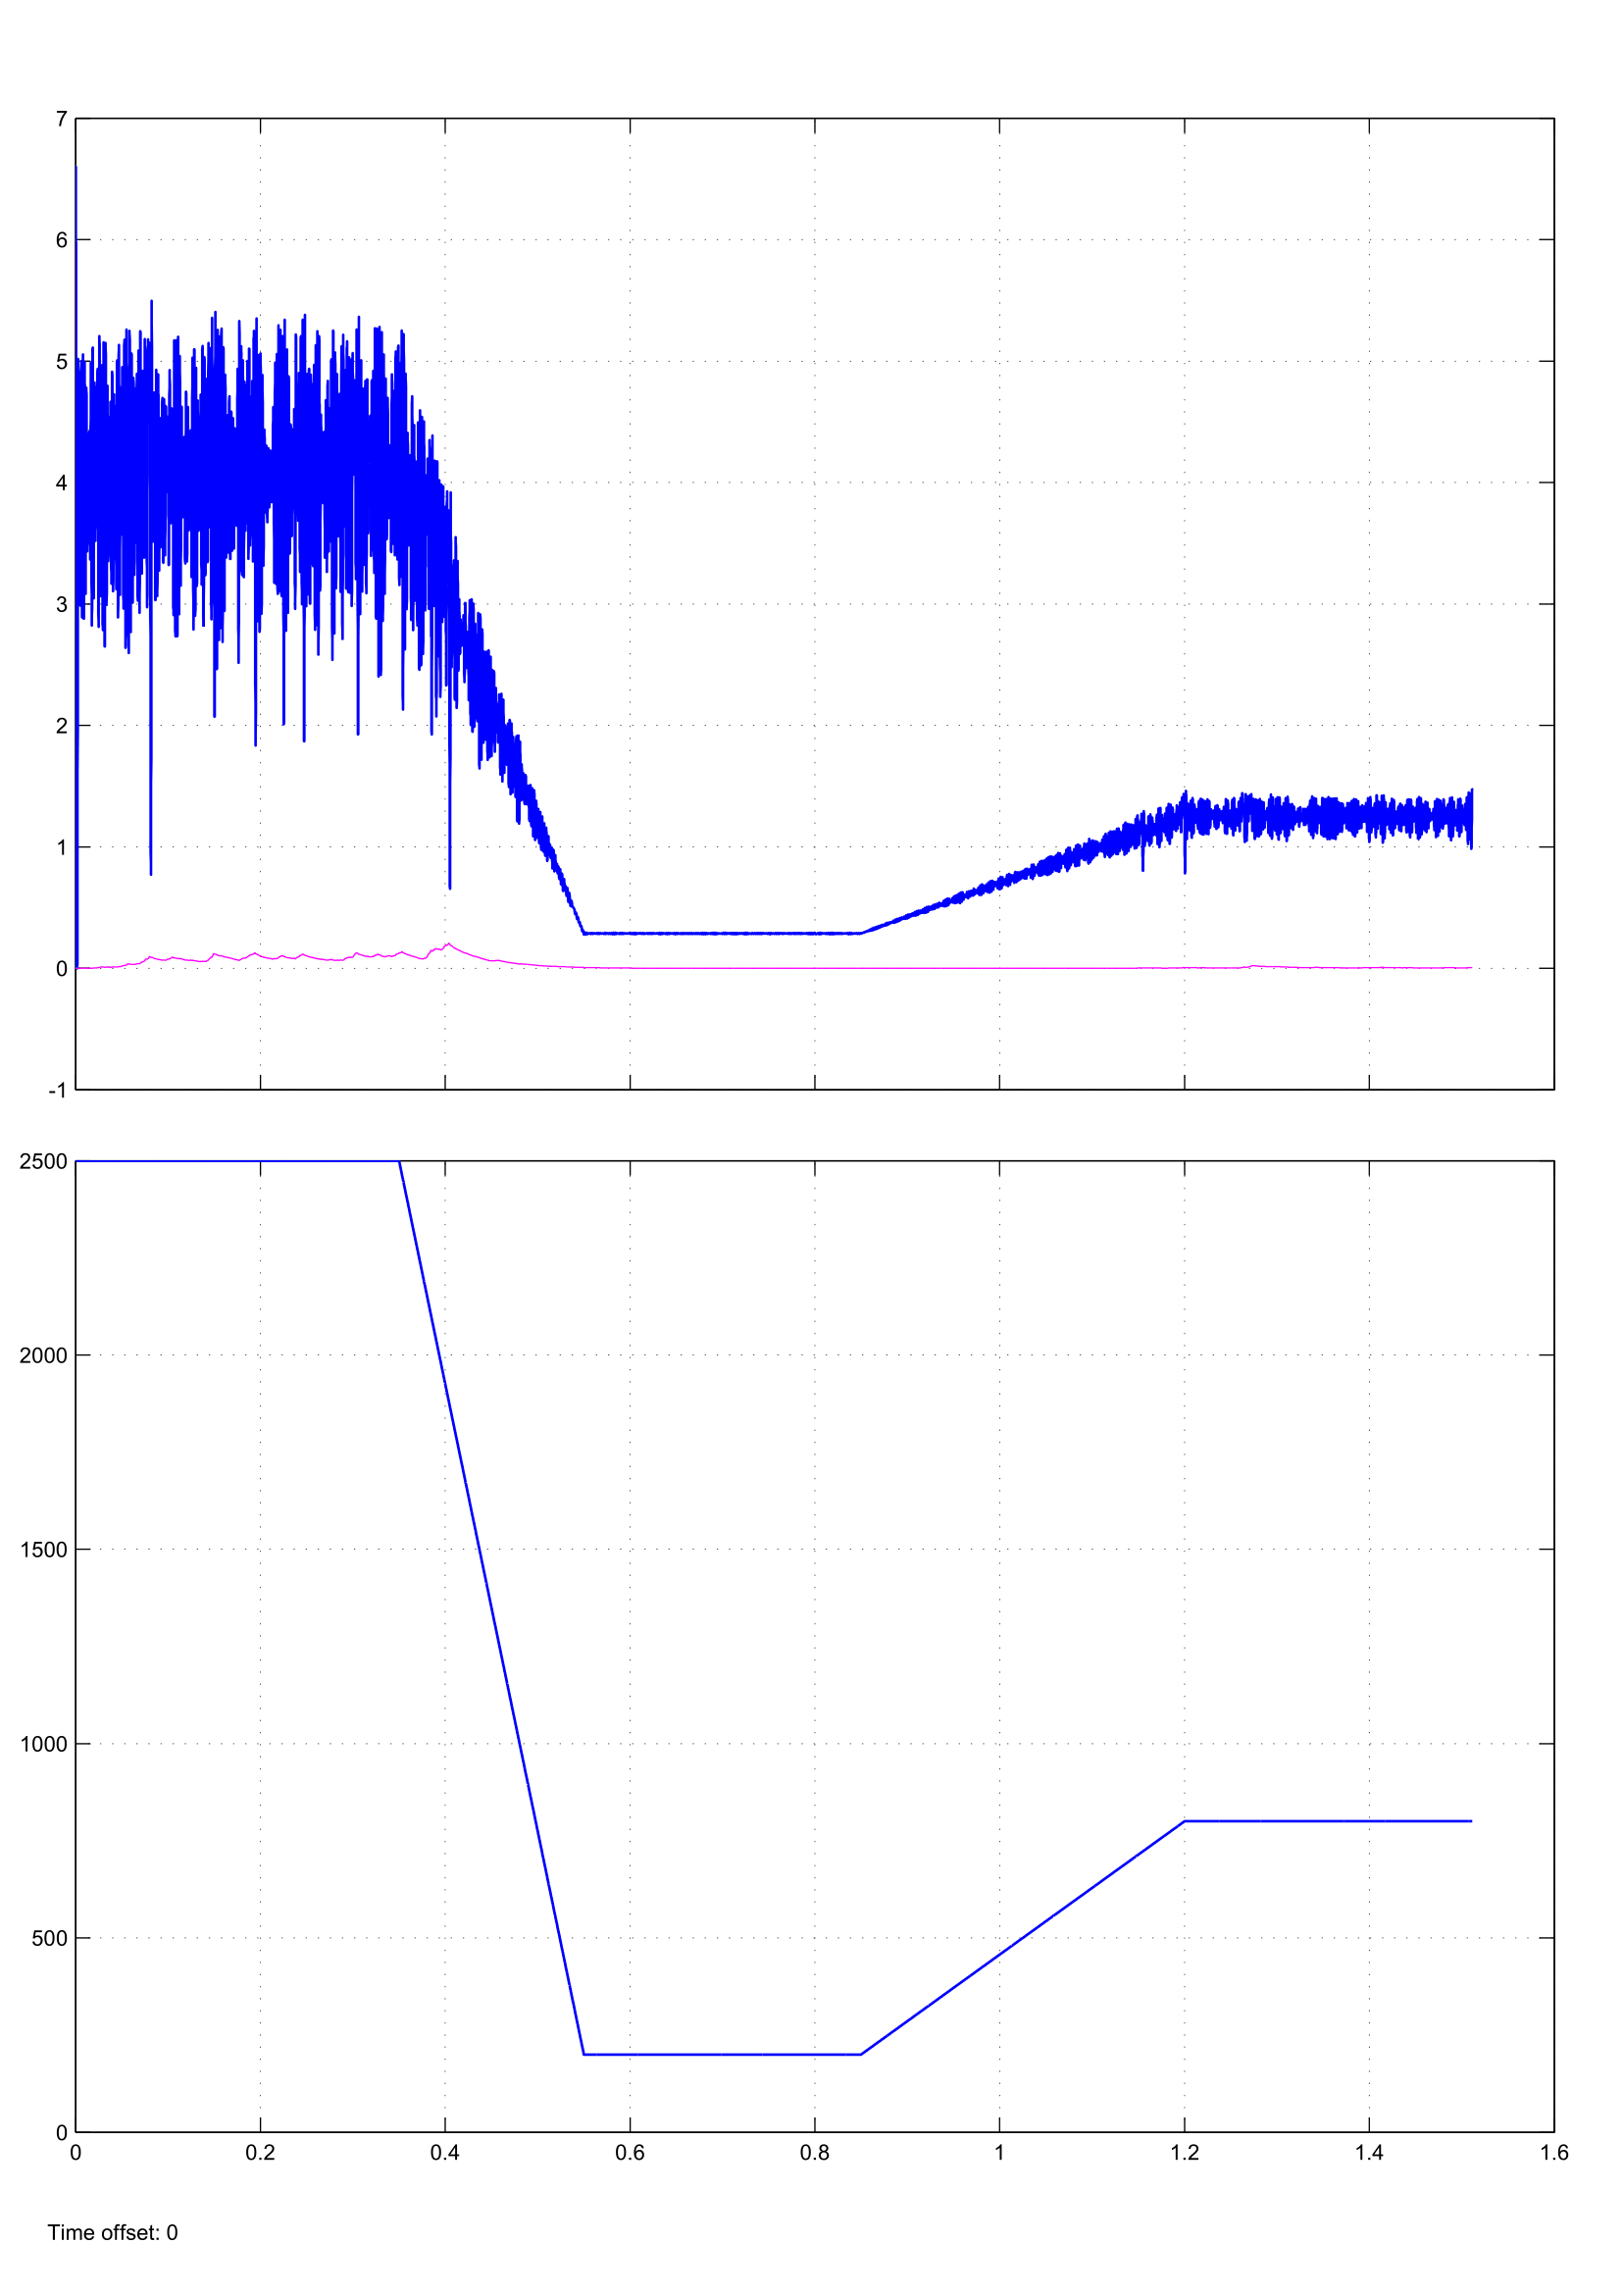
\includegraphics[width=\textwidth]{images/inC_stateflow_changing_lux-1}
		   \caption{Incremental Conductance Method on implementation  }
		   \label{fig:Inc_result}
	   \end{center}
  \end{figure}
 The underlying principle behind \ac{ICM}'s operation is the fact that the slope of the P-V curve is zero when \ac{MPP} is reached. The slope is negative to the right of \ac{MPP} and positive to the left.
 Depending on the direction of the slope $V\textsubscript{ref}$ is moved in steps left or right determined by the sign of the slope. When $V\textsubscript{MPP}$ is reached, the cell is held at that potential until a change in $\varDelta$$I\textsubscript{cell}$ is detected.\\
 
 Like in \ac{PnO}, the step size determines how fast \ac{MPP} is reached and its accuracy. Also like before it takes several hundred iterations before \ac{MPP} is reached, leading to longer locking on times - resulting in much lower efficiency. Fixed step size and the several hundred iteration need were the primary reasons \ac{PnO} method and \ac{ICM} were found unsuitable to be used with \ac{DSCs} for \ac{MPPT}. Another argument for not using the two algorithms is that for every iteration two sensors required to be turned, this coupled with the high number of iterations needed; adds up to quite a bit of power used in finding the optimal operating point.             
 
         
 \section{Fractional Open Circuit Voltage Method }
 
As explained in section ~\ref{sec:proposed_algo_sec}, although \ac{FOCV} method has several advantages in terms of simplicity, speed and number of sensors used; the greatest drawback of this method would be its inability of every achieving true \ac{MPP}. By assuming $K_{i}$ as a constant under different illuminations leads to slight loss of power but the simplicity of the circuit helps in reducing its power consumption, This seems to be a fine balance whose odds can be increased by choosing an appropriate value of $K_{i}$. Under simulations, \ac{FOCV} shows a lot of promise by being extremely fast in latching on to $V\textsubscript{MPP}$ with minimal iterations. However the power from the cell was always lower than expected. Since under indoor conditions \ac{DSCs} produce minuscule amount of power, any loss would seem significant. The graph for the simulation of\ac{FOCV} looks similar to the one in figure~\ref{fig:Frac_oc_result} on page~\pageref{fig:Frac_oc_result}, key difference being the power levels were lower.             

\section{Proposed Method }

Based on the learnings from simulations and experiments, it was apparent that the selected algorithms would not be the best fit for \ac{DSCs}. Section ~\ref{sec:proposed_algo_sec} makes clear the inner working of the routine. The results are divided into two parts.\\
	
	\begin{enumerate}
		\item Finding \ac{MPP} when the buffer is full.
		\item Locking on to $V\textsubscript{MPP}$ when look-up table is empty or when an out of range $V\textsubscript{OC}$ is detected.				
	\end{enumerate}
In the first condition, the sub-routine that is utilized behaves in a manner similar to \ac{FOCV} but deviates by dynamical varying the $K_{i}$ value based on the cell characteristics and past values.    
   \begin{figure}[H]
  	  \begin{center}
  		  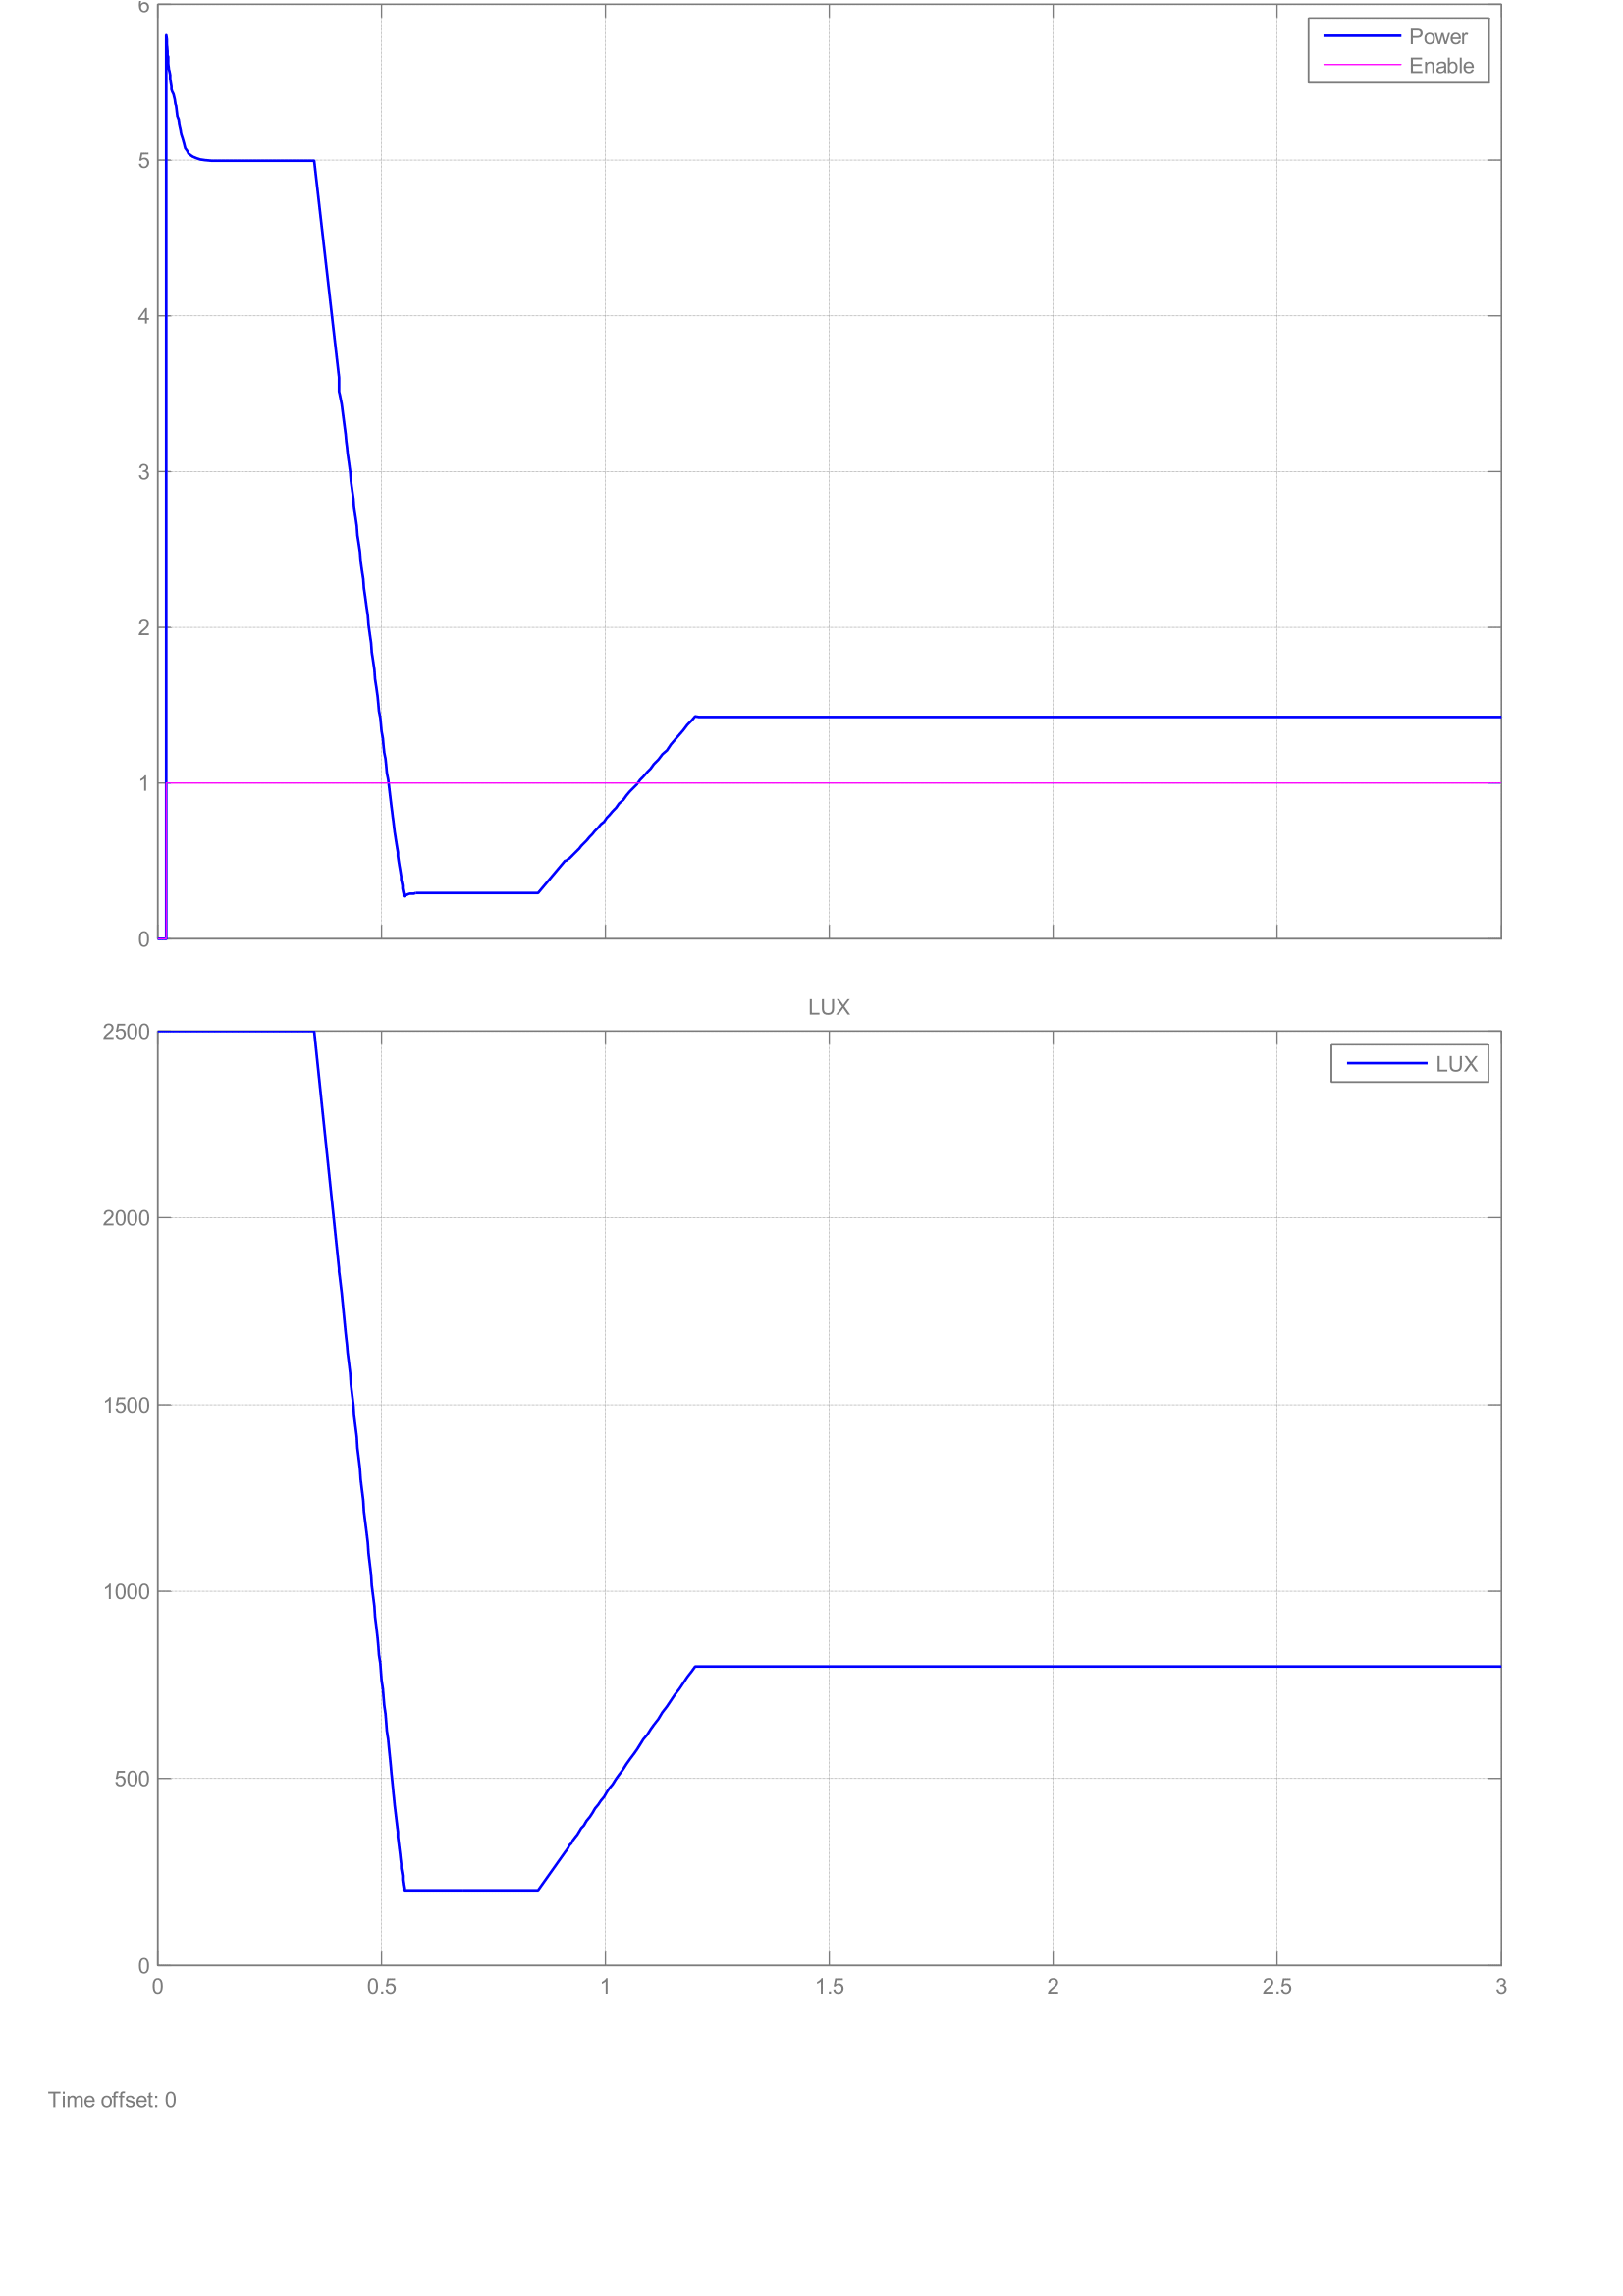
\includegraphics[width=\textwidth]{images/Proposed_algo-1}
  		  \caption{Proposed routine with full buffer, under similar light conditions as other algorithm}
  		  \label{fig:Frac_oc_result}
  	  \end{center}
    \end{figure}

The ability of the algorithm to latch-on to the optimal operating point at great speed is an advantage, greatly reducing the power wasted while searching for the \ac{MPP} (power lost due operating the cell on non-optimal potential and power lost due to the active circuitry while searching). The fact that only one sensor, a simple voltage sensing element, is activated for a fraction of a second is an added benefit. Under its typical use case, incident radiation is not expected to vary frequently or by a large degree meaning the \ac{MPPT} controller operates in this sub-routine for majority of the time.\\

For the case where the look-up table is not yet fully populated or when the cell encounters a Lux level that it has not encountered before, a different branch of the algorithm is called. This sub-routine employs \ac{GSSA} to find $V\textsubscript{MPP}$, the search window employed is dynamically chosen based on previous results so as to reduce the number of iterations required to reach the \ac{MPP}.\\

Under indoor-light conditions, gradual change of illumination is rarely encountered, what we do run up against is more discrete light levels in the form of turning on/off one or more light sources in a room. Granted sunlight streaming in from windows does follow a more gradational pattern, this can easily be incorporated in to the controller's design. These discrete lux levels are a perfect platform to demonstrate the speed at which \ac{GSSA} converges onto the \ac{MPP}.\\

Figure~\ref{fig:proposed_empty_lookup} on page~\pageref{fig:proposed_empty_lookup} depicts output of a controller subjected to discrete light levels starting from 2500 Lux down to 400 Lux. The plot enclosed in the red box is expanded in figure~\ref{fig:Zoom_proposed_empty_lookup} on page~\pageref{fig:Zoom_proposed_empty_lookup}. An enable signal (in pink) was added to indicate start of the search. It is worth noting the speed at which the search algorithm converges onto the Maximum power point. The number of iterations taken before \ac{MPP} was found, fell between 15 - 20, a far cry from the several hundred needed for \ac{PnO} or \ac{ICM}. This means that even if the cell were to be given a second worth of time to stabilise between iteration, the $V\textsubscript{MPP}$ would still be reached within 20 seconds. Consequently this also means the two sensors needed for measuring power would be used a lot fewer times compared to before. \\
       
                     
 \begin{figure}[H]
  \begin{center}
  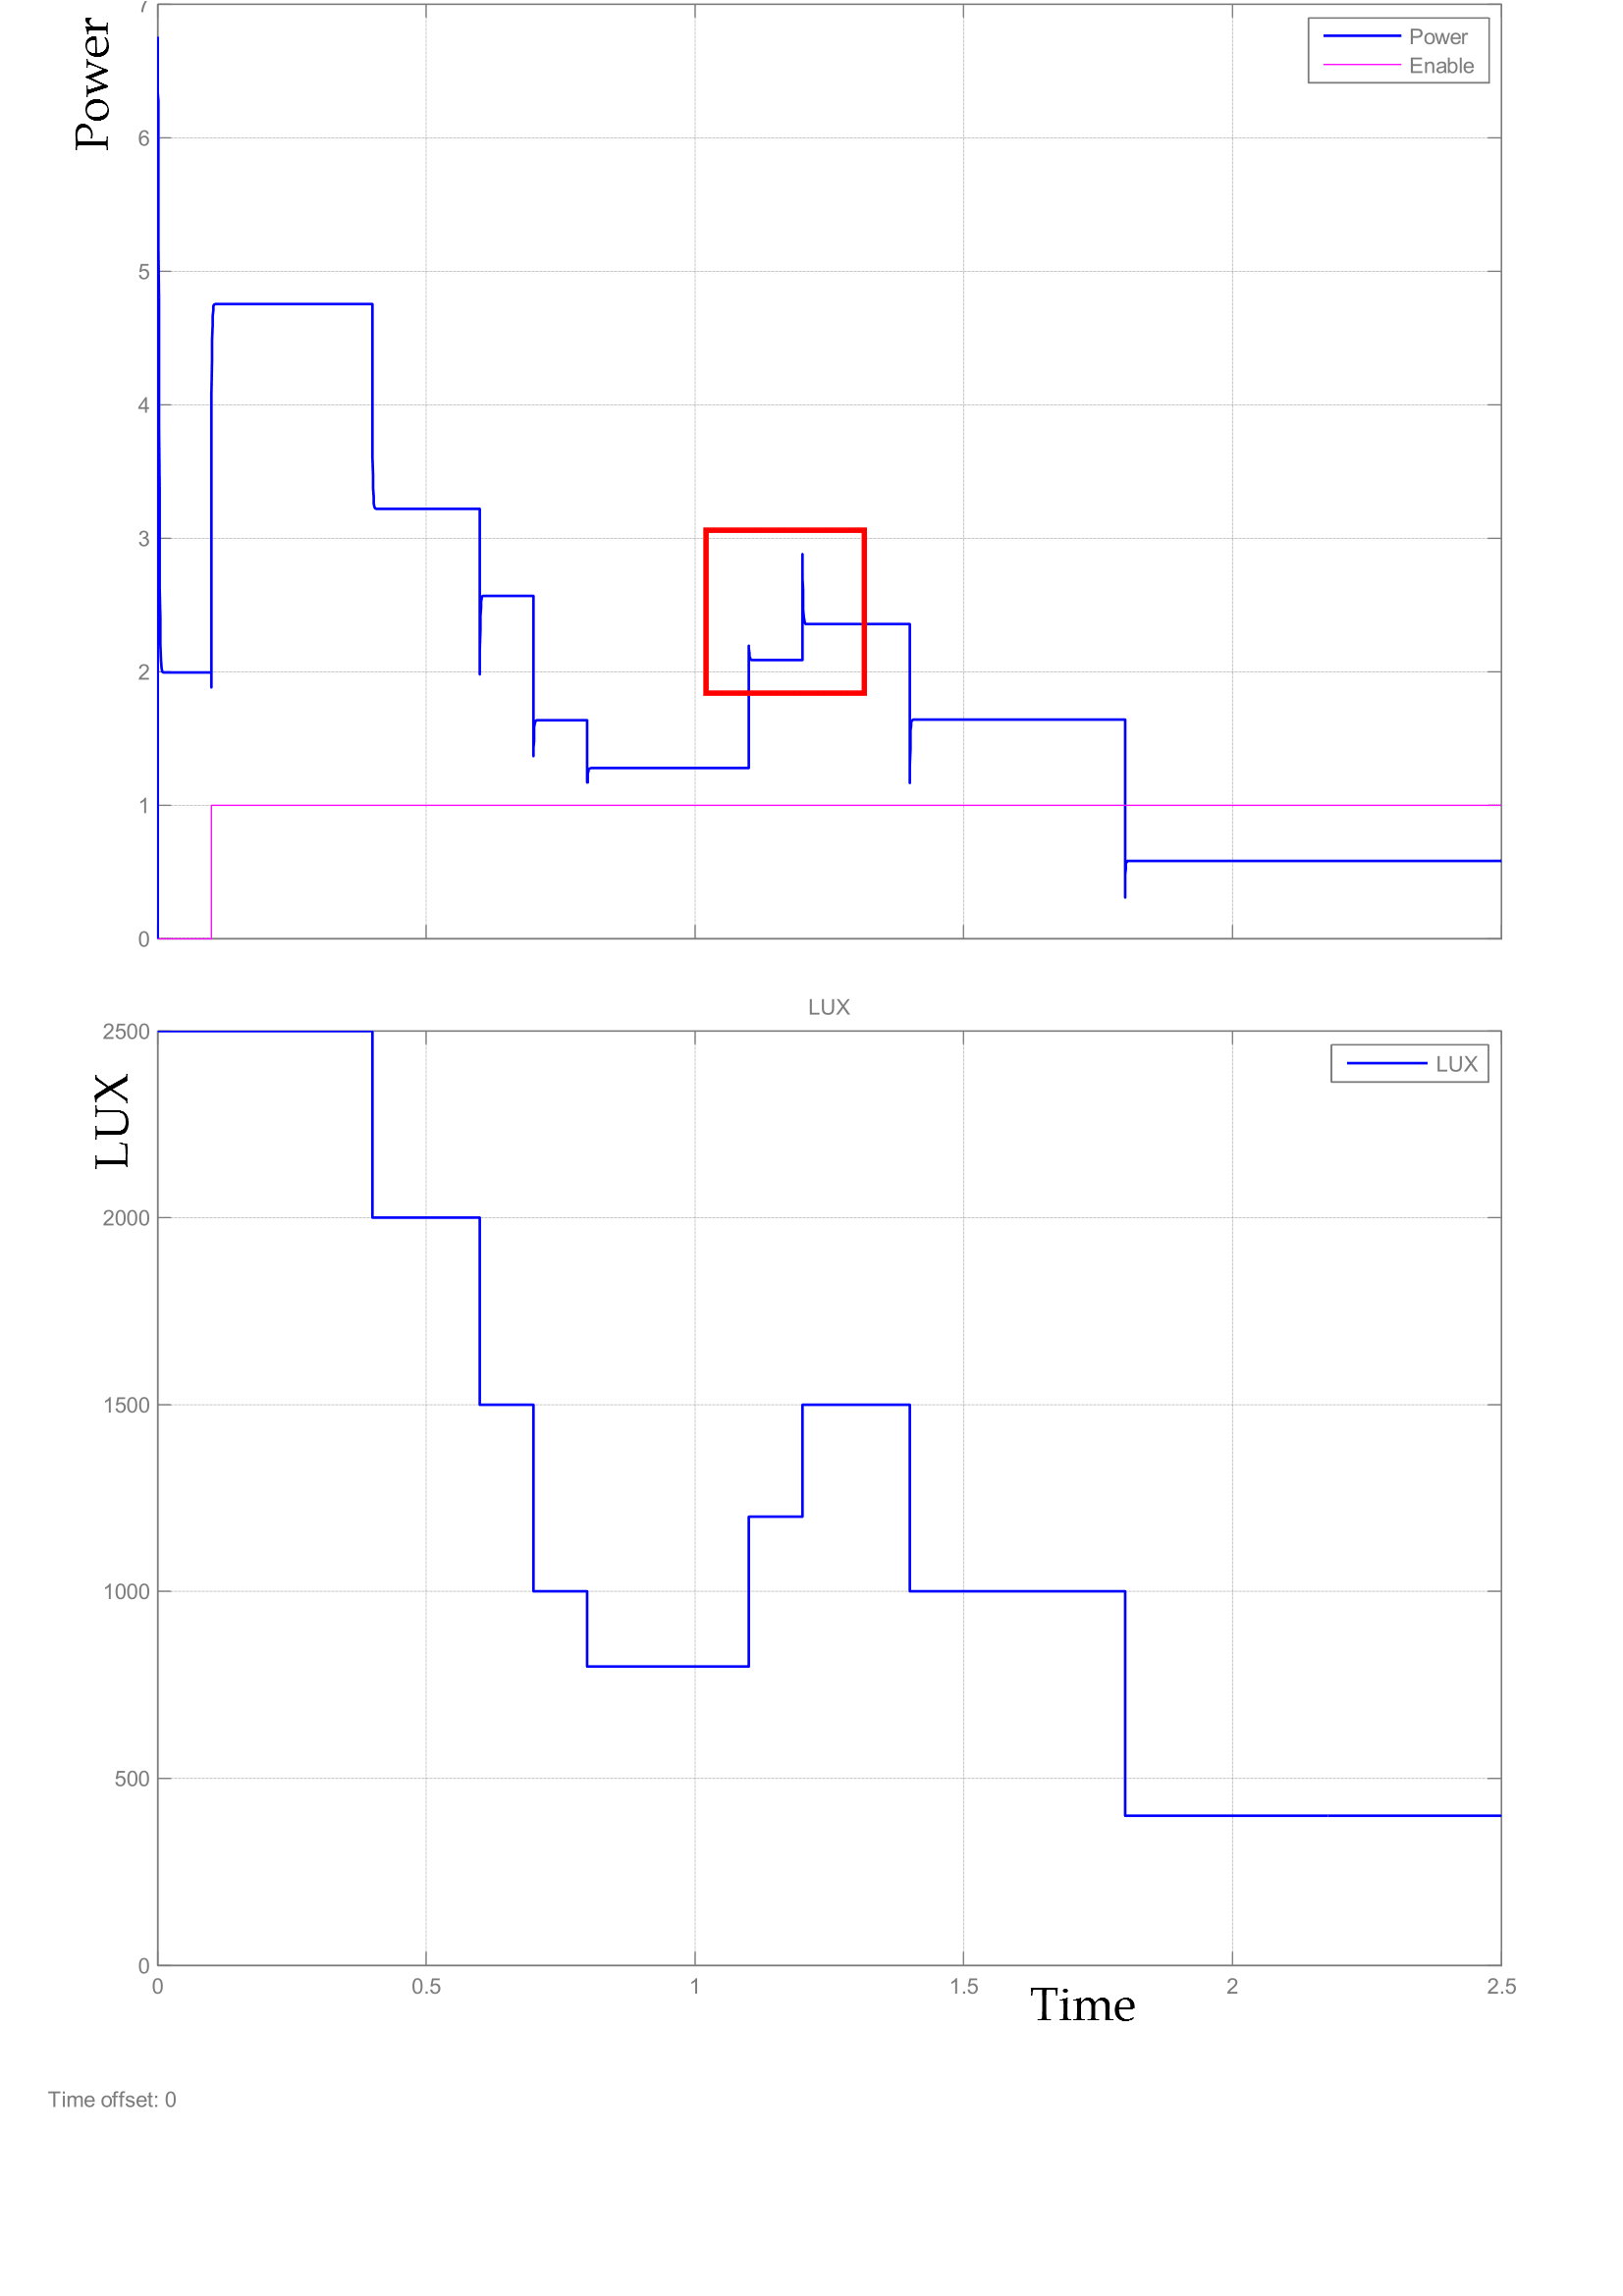
\includegraphics[width=\textwidth]{images/proposed_step_input}
  \caption{Proposed algorithm under rapidly varying light conditions with empty lookup tables }
  \label{fig:proposed_empty_lookup}
  \end{center}
  \end{figure}


 \begin{figure}[H]
  \begin{center}
  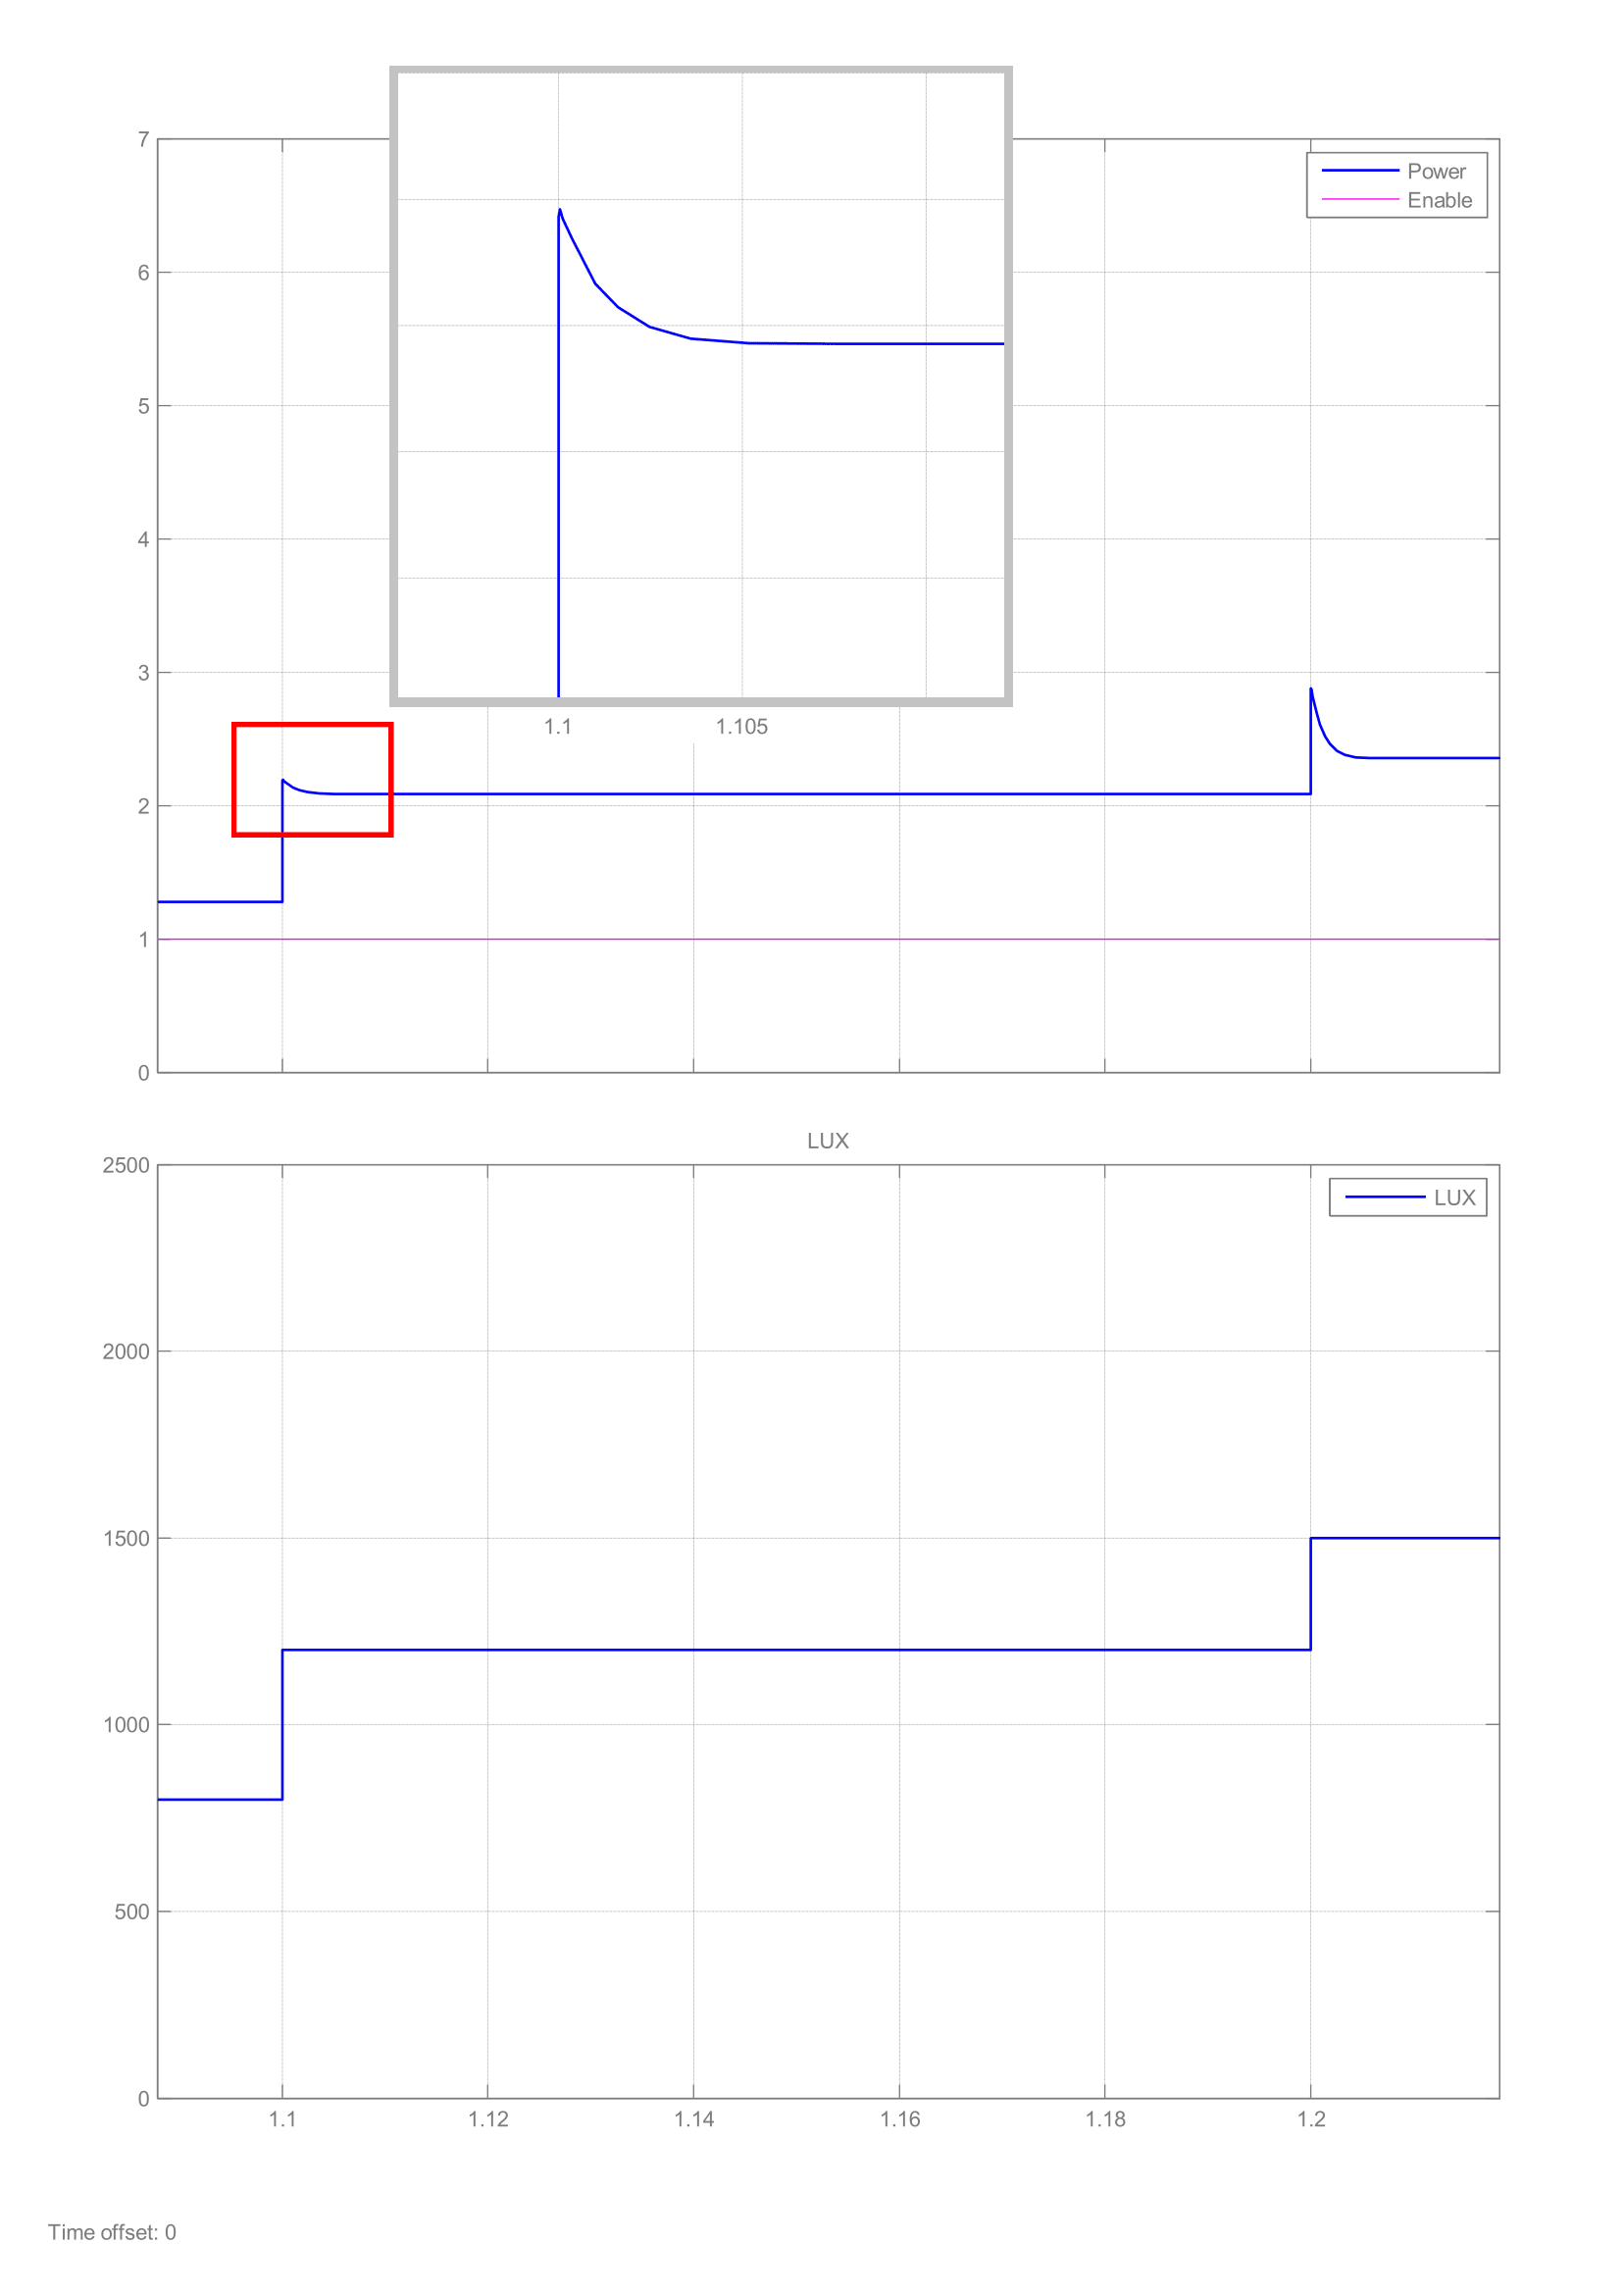
\includegraphics[width=\textwidth]{images/proposed_step_input_zoom-1(2)_pip}
  \caption{ expanded view of the graph in figure ~\ref{fig:proposed_empty_lookup}}
  \label{fig:Zoom_proposed_empty_lookup}
  \end{center}
  \end{figure}

\section{Comparison}
Outlined below is a comparison of the result obtained by subjecting the various algorithms under test to similar input conditions. 
\begin{center}
    \begin{tabular}{ | l | l | p{4cm} | p{4cm} |}
    \hline
    Algorithm & Sensors Required & Iterations (depending on step-size) & Time required to Lock on to MPP* \\ \hline
    \ac{PnO} & 2 & $~300 -400$ & $5-6$ min. \\ \hline
    \ac{ICM} & 2 & $~300 -400$ & $5-6$ min. \\ \hline
    \ac{FOCV} & 1 & 1 & 500 ms. \\ \hline
    Proposed algo. & 1 (majority) & 1  (Min) & 500 ms (Min)\\
    & 2 (Start-up) & 25 (Max) & 25 sec (Max).\\ \hline
   \end{tabular}
\end{center}
\textbf{*}\textit{ Assuming 1 sec rest between iterations.}


  




